\documentclass[11pt]{beamer}
\usetheme{Goettingen}
\usepackage[utf8]{inputenc}
\usepackage{amsmath}
\usepackage{amsfonts}
\usepackage{amssymb}
\usepackage{graphicx}
\usepackage{hyperref}
\author{Alex Heilman}
\title{Crystal Hypergraph Neural Networks}
\subtitle{A Universal Framework for Material Machine Learning}
%\setbeamercovered{transparent} 
%\setbeamertemplate{navigation symbols}{} 
%\logo{} 
%\institute{} 
%\date{} 
%\subject{} 

\newenvironment{boxed2}
    {\begin{center}
    \begin{tabular}{|p{0.95\textwidth}|}
    \hline\\
    }
    { 
    \\\\\hline
    \end{tabular} 
    \end{center}
    }


\begin{document}

\begin{frame}
\titlepage
\end{frame}

%\begin{frame}
%\tableofcontents
%\end{frame}

\begin{frame}{Overview}

$\bullet$ Crystal Graphs Lack Higher Order Geometrical Info of Crystal Structure \pause -- Motifs!

\vspace{.7cm}\pause

$\bullet$ Use Hypergraphs, with Motif Info/Shapes Encoded as Higher Order Hyperedge (Hedge) Attributes

\vspace{.7cm}\pause

How to handle these?\pause

\medskip\pause

$\bullet$ Convert Hypergraphs into 'Relatives' (Hetero) Graph  to Feed into Usual (Hetero) Graph Neural Networks, like CGCNN

\medskip\pause

$\bullet$ Apply a novel convolutional structure adaptable to variable size hyperedges


\end{frame}

\section{Crystal Graphs}
\begin{frame}{Usual Crystal Graph Construction \small(a la CGCNN)}

$\bullet$ Atoms are nodes, with initial node features determined by atomic properties

\medskip

\begin{center}

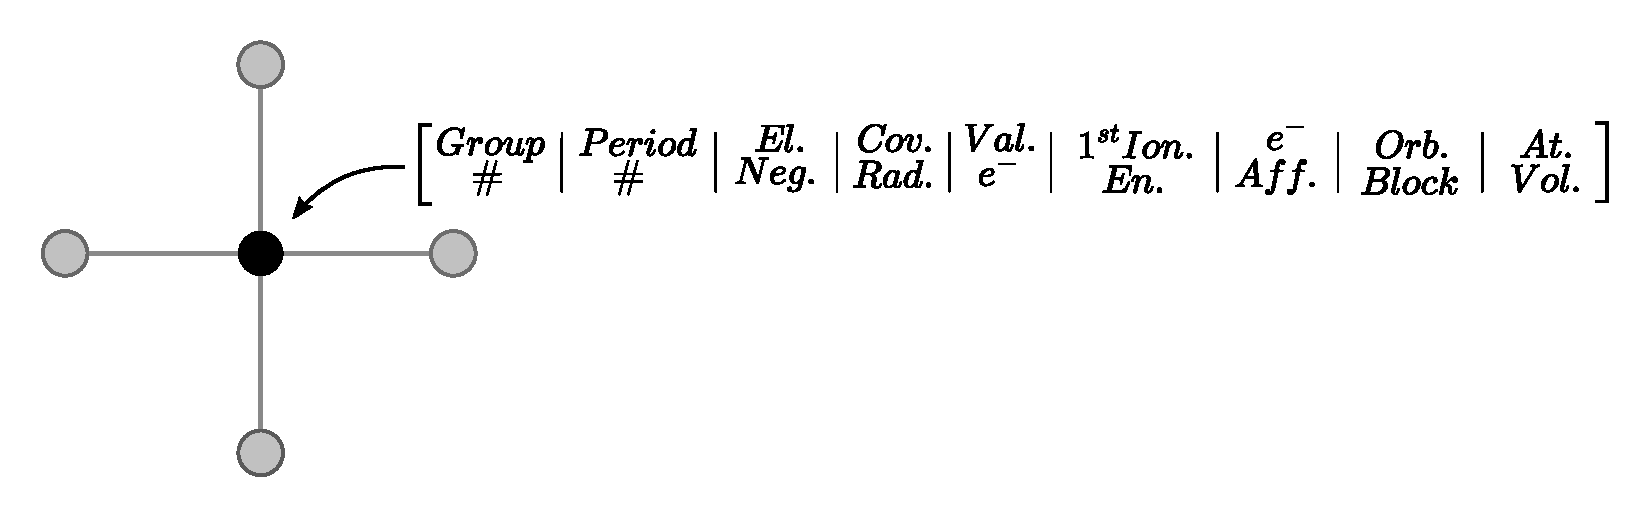
\includegraphics[scale=0.3]{atom_feat.pdf}

\end{center}
\end{frame}

\begin{frame}{Crystal Graphs cont. I}

$\bullet$ Edges are determined by distance cutoff (4 Ang.) and maximum number of neighbors (12)

\begin{center}
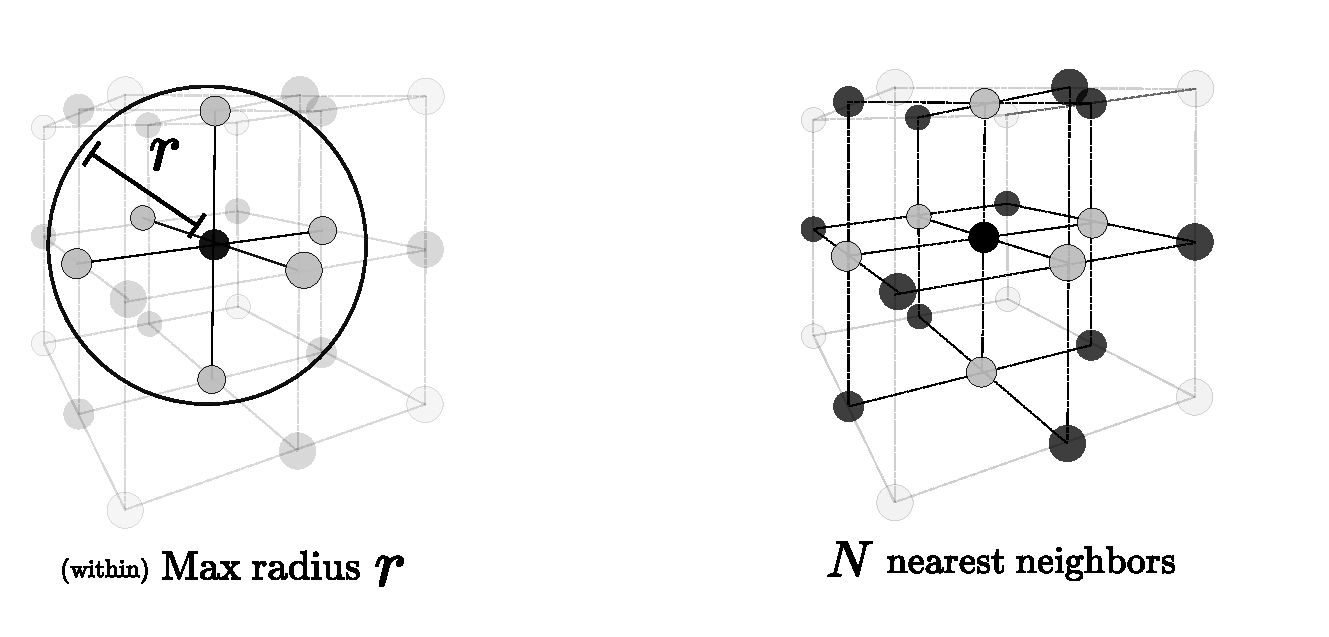
\includegraphics[scale=0.45]{ex_bondcriteria.pdf}
\end{center}
\end{frame}

\begin{frame}{Crystal Graphs cont. II}
Edge attributes then are a Gaussian distance expansion

\begin{center}
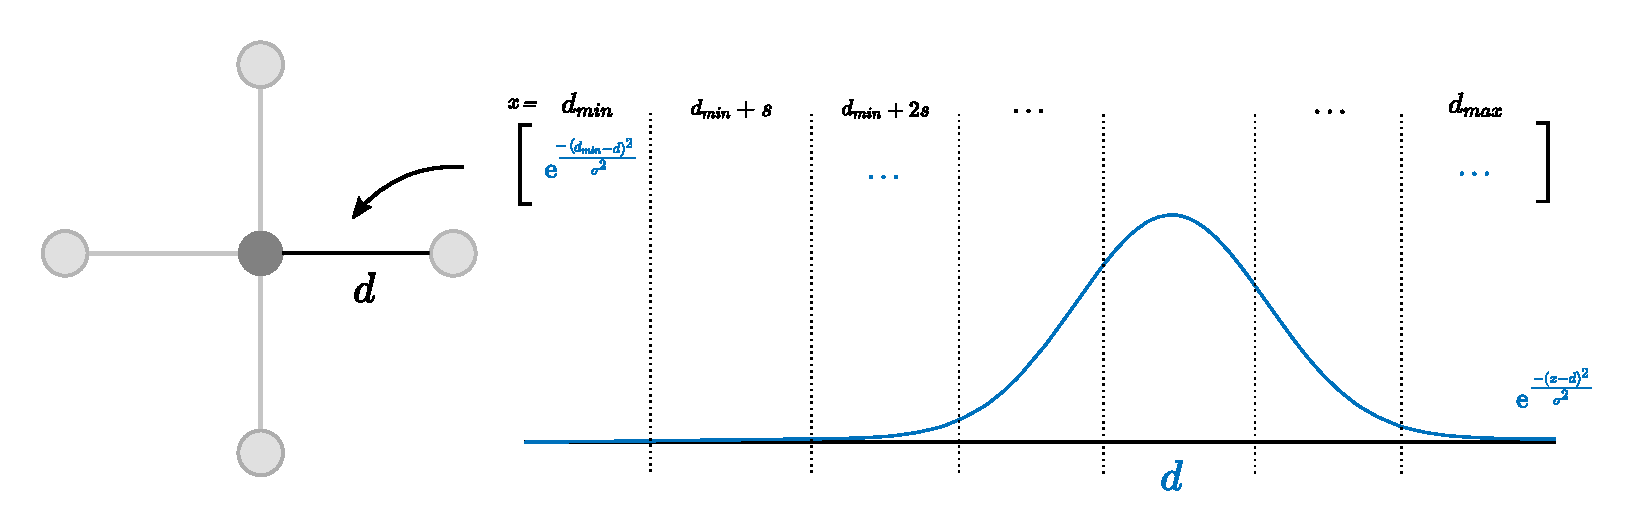
\includegraphics[scale=0.33]{bond_feat.pdf}
\end{center}
\end{frame}

\begin{frame}{Graph Limitations}
Problem: Only encodes distances between atoms!

\vspace{.7cm}

Recent works: Atomistic Line graph generates a second graph (the line graph) associated with the crystal graph

\vspace{.4cm}

In line graph, nodes represent edges and line graph edges represent overlapping/connected edges.

\vspace{.4cm} 

Allows for encoding of angle information (between bonds) as edge attributes in line graph
\end{frame} 

\section{Crystal Hypergraphs}
\begin{frame}{Hypergraphs}
Hypergraphs allow us to have edges containing more than (or less than) two nodes.

\vspace{.5cm}

Natural way to encode features with higher order structure, where hypergraph nodes still represent atoms of underlying crystal structure.

\vspace{.5cm}

Can treat all different order structures on equal footing: each has a corresponding hyperedge with a feature
\end{frame}

%\begin{frame}{Atom Hedges}
%We first generate singleton hedges for each atomic site (the reason will be apparent later)

%\vspace{0.5cm}

%\begin{center}
%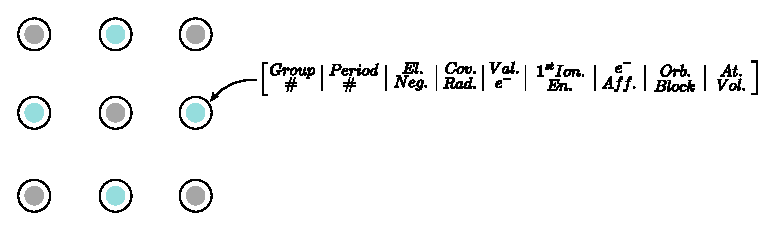
\includegraphics[scale=0.73]{singleton.pdf}
%\end{center}

%\end{frame}

\begin{frame}{Pair Hedges}
We first generate pair-wise (second order) hyperedges, equivalent to regular crystal graph edges.

\vspace{0.5cm}

\begin{center}
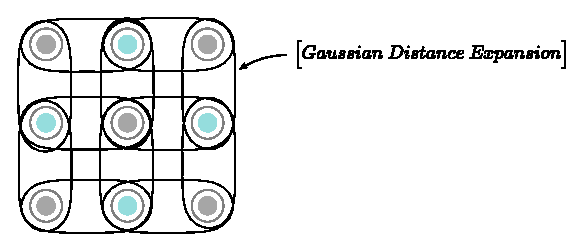
\includegraphics[scale=0.73]{pair.pdf}
\end{center}

\end{frame}

\begin{frame}{Motif Hedges}
Wish to include higher order geometrical information of crystal structure. Motifs have important information!

\vspace{0.5cm}\pause

Generate motif hedges, associate local structure order parameters (describing local environment's shape) as feature.

\vspace{0.5cm}

\begin{center}
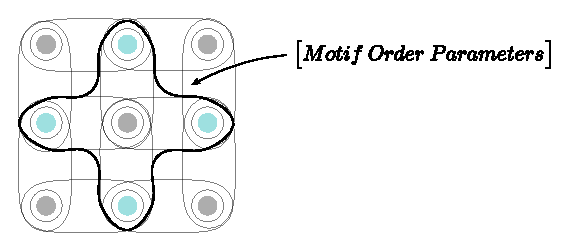
\includegraphics[scale=0.73]{motif.pdf}
\end{center}
\end{frame}


\begin{frame}{Hypergraph Convolutions: Two Approaches}
First idea: form a relatives \textbf{graph} corresponding to the original hypergraph, allowing us to use the usual graph convolution functions

\vspace{2cm}

Second idea: apply a novel \textbf{hypergraph convolution} directly to the hypergraph

\end{frame}

\begin{frame}{Relatives Graph Construction}
We term this inherited graph from the hypergraph the relatives graph, since connected nodes are related structures.
\begin{center}
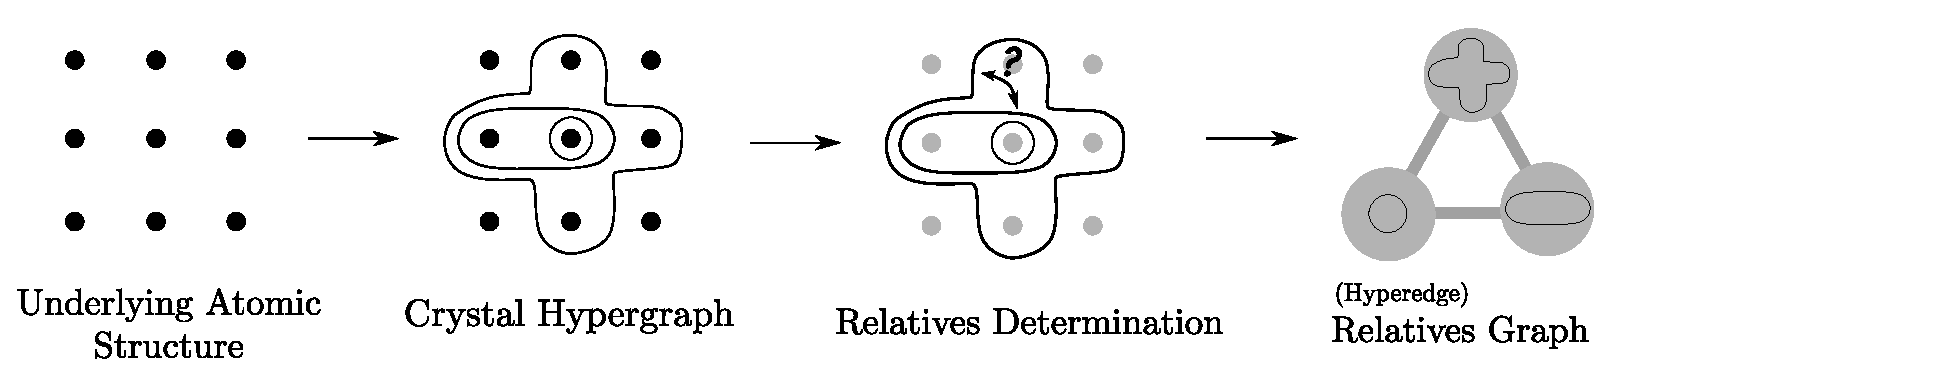
\includegraphics[scale=0.33]{relgraph_workflow_horiz.pdf}
\end{center}

Note that this is naturally a heterogeneous graph, in that there are different types of nodes
\end{frame}

\begin{frame}{Relatives Graph Convolution}
Applying arbitrary graph convolutional operators to this relatives graph essentially leaves us with the following form for the layer-to-layer updating node-wise.
\begin{align*}
x_i\rightarrow x_i&+f_{xx}(x_i\oplus x_j)\\
				  &+f_{xb}(x_i\oplus b_j)\\
				  &+f_{xm}(x_i\oplus m_j)\\
\end{align*}
Each different order structure has it's own (directional) update function.

\medskip

Unfortunately, this seems to hinder performance. Perhaps this occurs since neighboring node features may not interact as strongly without being concatenated in the message forming phase.
\end{frame}

\begin{frame}{Hypergraph Message Passing}
In the case of a hypergraph, the neighborhood of nodes relevant to each message are now a set (instead of the single neighboring node feature of classic MPNNs)

\begin{gather*}
m_v^{t+1}=\sum_{h_j\in \mathcal{N}(v)} M_t(n_v^{t},\underbrace{h_j^{t},\lbrace  n_w^t \vert n_w \in h_j }_{e_{vw},n_w}\rbrace)\\
\\
n_v^{t+1}=U_t(n_v^t,m_v^{t+1})\\
\\
\hat{y}=R(\lbrace n_v^T\rbrace)\\
\end{gather*}

The rest of the structure may essentially remain the same

\end{frame}

\begin{frame}{Hypergraph Convolution}
To deal with the variable sized neighborhoods of features, we simply aggregate the neighborhood features in the message passing phase, so that we essentially have the following form of convolution:
\begin{align*}
x_i \rightarrow x_i &+ f_b(x_i\oplus e_{ij} \oplus \text{AGG}(\lbrace x_i, x_j\rbrace))\\
&+ f_m(x_i\oplus m_{j} \oplus \text{AGG}(\lbrace  n_w^t \vert n_w \in m_j \rbrace))
\end{align*}

\end{frame}

\begin{frame}
Current Problems/Outlook:

\medskip

$\bullet$ CGConv baseline should line up better with CGCNN from the original github

\medskip

$\bullet$ What other features/structure orders should be included?

\medskip

$\bullet$ What is the best balance between efficiency and efficacy? Do we even need pairwise edges or motif edges?

\medskip 

$\bullet$ Novel use case: apply to scenarios where motifs are effectively smallest structural unit of crystalline system (ceramics)
\end{frame}

\begin{frame}{{\small Other Project:} Spherical Harmonic Decomposition of Elastic Tensor}

\end{frame}

\end{document}